\begin{center}
\Huge
Aflevering 2
\end{center}
\section*{Opgave 1}
\stepcounter{section}
To funktioner $f$ og $g$ er givet ved henholdsvist
\begin{align*}
f(x) &= x^2+1,\\
g(x) &= -2x^2-7x+10.
\end{align*}
\begin{enumerate}[label=\roman*)]
\item Bestem skæringspunkterne $A$ og $B$ mellem funktionerne $f(x)$ og $g(x)$.
\item Bestem ligningen for den rette linje $l$, der går gennem punkterne $A$ og $B$. 
\item Linjen $m$ givet ved ligningen 
\[ m: \ y = x
\]
afgrænser sammen med linjen $l$ og $x$-aksen et trekantet område. Bestem arealet af dette område.
\end{enumerate}

\section*{Opgave 2}
Lad $f$ være givet ved 
\begin{align*}
f(x) = x^5-4x^4+3x^3-2x^2+x.
\end{align*}
\begin{enumerate}[label=\roman*)]
\item Bestem den afledede funktion $f'$ af $f$.
\item Bestem ligningen for tangenten for $f$ i punktet $(1,f(1))$.
\item Er der andre tangenter til $f$, der er parallelle til denne tangent? Bestem i så fald deres ligning.
\end{enumerate}

\section*{Opgave 3}
Lad os sige, at vi har et polynomium $p(x) = a_nx^n + a_{n-1}x^{n-1}+\cdots+a_1x+a_0$.
\begin{enumerate}[label=\roman*)]
\item Hvor mange led har polynomiet $p$?
\item Hvis vi differentierer $p$, så forsvinder leddet $a_0$, og konstantleddet for $p$ hedder så $a_1$. Bestem hele $p'$.
\item Hvis vi differentierer polynomiet en gang til, så vil leddet $a_1$ også forsvinde. Hvor mange gange skal vi differentiere $p$ for at hele polynomiet forsvinder?
\end{enumerate}

\section*{Opgave 4}
Der skal bygges en pyramide med så stort rumfang som muligt. Der er kun sten nok til at overfladen på pyramiden kan være 2km$^2$. Rumfanget af en pyramide med 4 sider er givet ved $R = \frac{hbl}{3}$, hvor $l$ er længden, $h$ er højden og $b$ er bredden. Vores pyramide skal have kvadratisk bund. Den kan ses på Fig. \ref{fig:pyramide}
\begin{figure}[H]
\centering
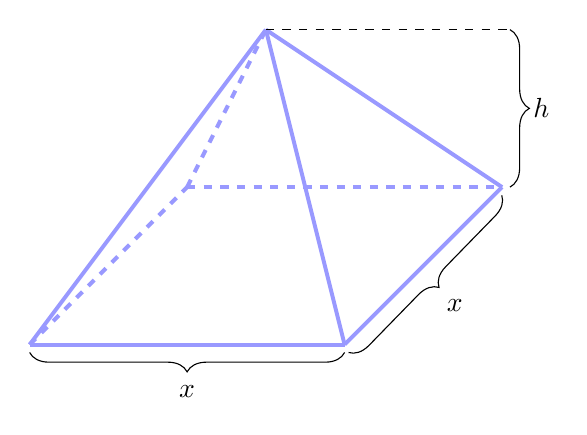
\begin{tikzpicture}
\draw[line width = 0.5mm,  color = blue!40] (0,0) -- (4,0);
\draw[line width = 0.5mm,  color = blue!40] (0,0) -- (3,4);
\draw[line width = 0.5mm,  color = blue!40] (4,0) -- (3,4);
\draw[line width = 0.5mm,  color = blue!40] (6,2) -- (3,4);


\draw[line width = 0.5mm,  color = blue!40] (4,0) -- (6,2);

\draw[line width = 0.5mm, dashed,  color = blue!40] (0,0) -- (2,2);
\draw[line width = 0.5mm, dashed,  color = blue!40] (2,2) -- (6,2);
\draw[line width = 0.5mm, dashed,  color = blue!40] (2,2) -- (3,4);
\draw[line width = 0.2mm, dashed] (3,4) -- (6.1,4);


\draw [decorate,decoration = {brace,mirror,amplitude = 7pt}] (0,-0.1) --  (4,-0.1);
\draw [decorate,decoration = {brace,mirror,amplitude = 7pt}] (4.05,-0.1) --  (6,1.9);
\draw [decorate,decoration = {brace,mirror,amplitude = 7pt}] (6.1,2) --  (6.1,4);

\node at (2,-0.6) {$x$};
\node at (5.4,0.5) {$x$};
\node at (6.5,3) {$h$};
\end{tikzpicture}
\caption{Pyramide med kvadratisk bund}
\label{fig:pyramide}
\end{figure}
Der skal ikke være nogen bund i pyramiden. 
\begin{enumerate}[label=\roman*)]
\item Bestem et udtryk for rumfanget af pyramiden. 
\item Forklar, hvorfor overfladearealet af en af de fire sidetrekanter er givet ved 
\begin{align*}
\frac{x}{2}\sqrt{\frac{x^2}{4}+h^2}.
\end{align*}
Brug dette til at bestemme et udtryk for det samlede overfladeareal. 
\item Udnyt, at det samlede overfladeareal skal være 2km$^2$, og brug dette til at bestemme et udtryk for rumfanget, der kun afhænger af $x$. Plot dette udtryk. 
\item Bestem nu det $x$, der optimerer rumfanget af pyramiden. 
\end{enumerate}

\section*{Opgave 5 \large (uden hjælpemidler)}
En bestemt væske stilles i et rum. Temperaturen af væsken $T(t)$ i $^\circ C$ som funktion af tiden $t$ i minutter er tilnærmelsesvist bestemt ved udtrykket 
\begin{align*}
T(t) = 120e^{-0.02t}.
\end{align*}
\begin{enumerate}[label=\roman*)]
\item Hvilken væksttype aftager temperaturen af væsken med?
\item Hvad er temperaturen til tiden $t=0$? 
\item Hvad er temperaturen i rummet, væsken stilles i?
\item Bestem væksthastigheden for temperaturfaldet. Hvad er væksthastigheden efter 20 minutter?
\item Hvornår aftager temperaturen hurtigst?
\item Hvad er halveringstiden for $T$?
\end{enumerate}
